\section{Analyse}
Der er blevet lavet en række diagrammer over de forskellige detaljeret brugsmønster.\\
Der er to forskellige typer af analyse diagrammer, der er de dynamiske og de statisk.

\subsection{Statiske side af analysen}
Klasse diagrammet består af 9 klasser: Afdeling, Sag, Afgørelsesbrev, Ydelse, Person, Sekretær, Sagsbehandler, Afdelingsleder og Borger. De to mest centrale klasser i diagrammet er Afdeling og Sag, som skaber grundlaget for systemet. \\ \\
Afdeling består af attributterne ”navn” og ”afdelingsID”, som blev valgt for at muliggøre identifikationen af et bosted. Klassen er central for systemet da den skal bruges til at administrere dem som arbejder i en afdeling og hvilke sager de er ansvarlige for. \\ \\
Sag er en klasse, som består af attributterne ”sagsnummer”, ”afgørelse” og ”formular”, samt metoden ”hentOplysninger()”. Klassen udgør omdrejningspunktet i arbejdet med sagsbehandling, da Sag klassen skal bruges i forbindelse med behandling af borgere. Attributten, ”formular”, repræsentere de dokumenter der skal udfyldes, i følge VUM (voksenudredningsmetoden), af personalet f.eks. sagsbehandler. \\ \\
Sag er forbundet til Afdeling for at indikere at en sag behandles i en specifik afdeling.\\
Ydelse er en klasse som repræsenterer hvilke botilbud og lignende som tildeles en borger ud fra deres behov. Ydelse er forbundet til Sag, da den tildeles baseret på en vurdering af en specifik sag. En borger kan modtage flere ydelser, men disse ydelser er alle baseret på de specifikke sager som berør den enkelte borger.\\ \\
Borger klassen repræsenterer en person som skal registreres i systemet for at modtage et givent tilbud. Borger klassen har attributten ”cpr-nummer”, som bruges til at identificere den borgeren. Yderligere arver Borger klassen fra Person, som giver attributten ”navn”.\\ \\
\begin{figure}
  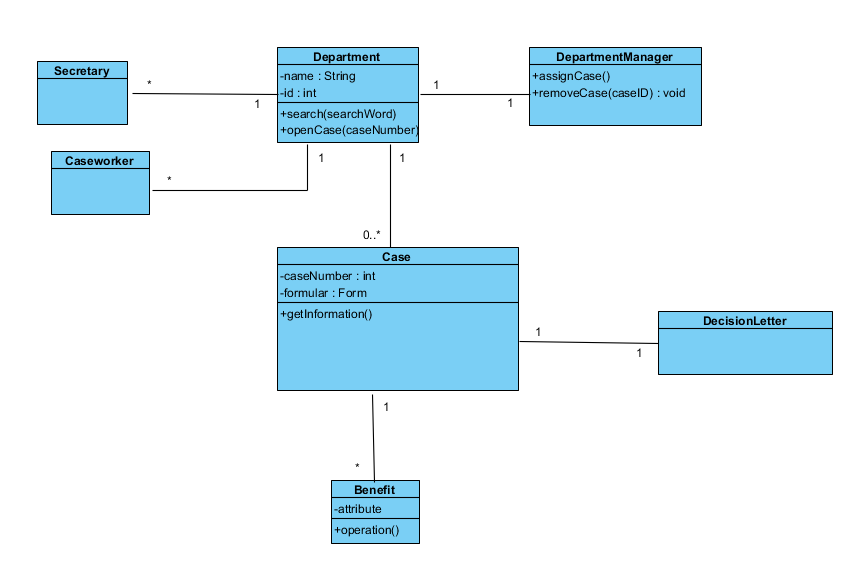
\includegraphics[width=\linewidth]{./PNG/analyseKlasseDiagram.PNG} 
  \caption{Analyse klasse diagram.}
  \label{fig:AKlasse}
\end{figure}

